\setcounter{figure}{0}
\setcounter{table}{0}
\section{Android平台开发相关技术简介}

\subsection{Android系统简介}
Android系统是由Google公司开发的一款主要面向触摸屏设备的直接控制式开源操作系统。该系统基于Linux内核,可运行在基于32位或64位ARM架构、x86架构和MIPS架构的设备上。目前Android系统已经广泛应用于智能手机、平板电脑、笔记本电脑、智能电视和一些可穿戴式设备上。近年来,Android系统的市场占有量持续领先其他同类型智能操作系统,是一款便于使用、便于开发的操作系统。
\begin{figure}[htbp]
 \centering
        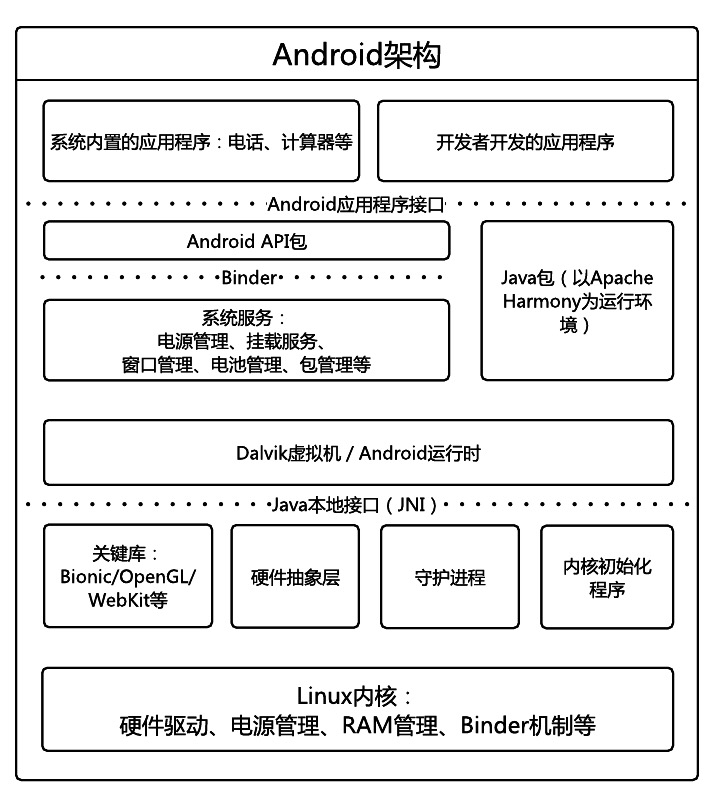
\includegraphics[width=0.5\columnwidth]{fig2-1.png}
        \caption{
                \label{fig2-1}
                Android系统架构
        }
\end{figure}

Android系统由Linux内核及底层组件、Dalvik虚拟机及运行时环境、系统服务、应用程序框架和应用程序四部分组成,其详细系统结构如图\ref{fig2-1}所示。Linux内核中包含Wakelocks、Binder、RAM Console等底层驱动和IPC/RPC机制。正是这些底层驱动实现了Android系统对音频、摄像头、显示、蓝牙、GPS等外围设备的支持。在该内核上还运行着一些关键库,如Bionic标准C语言库(libc.so、libstdc++.so、libdl.so等)、libhardware.so硬件抽象层、libbinder.so Binder标准库等。这些库函数通过Java本地接口和Dalvik虚拟机进行沟通。Dalvik虚拟机是一种针对嵌入式系统设计的Java虚拟机,在更加节省运行所需空间的同时,还保证了程序运行的效率(这得益于Dalvik包含的Just-in-Time编译器可以将程序直接转换为二进制指令后运行)\cite{yaghmour_embedded_2013}。系统服务为Android应用提供了与硬件抽象层沟通的方法,这些服务既有用Java语言实现的,也有用诸如C、C++等其他语言实现的。当一个应用程序需要调用系统服务时,它首先从服务管理器查得需要调用的系统服务的句柄,然后通过Binder获得该系统服务并且使用它(比如调用其中的某个方法)。最上层、也是最贴近用户的Android应用程序提供了人机交互接口,“计算器”、“录音机”等应用程序——也即人们平时所称的APP——均属于应用程序。

\subsection{Android系统蓝牙功能介绍}

蓝牙(Bluetooth)技术是一种基于2.4GHz频段设备的射频通讯标准,使用蓝牙技术传输数据的功耗更低,成本小,易于使用\cite{bluetooth_sig_inc_bluetooth_????}。

\subsubsection{蓝牙串口协议简介}

蓝牙串口协议(Serial Port Profile,SPP)允许两台支持蓝牙技术的设备通过RFCOMM协议建立起虚拟的RS232串口传输通道\cite{riku_mettsla_serial_2012}。一台蓝牙设备可以选择性地兼容蓝牙技术中若干协议的某几种,若要使用SPP协议传输数据,两台蓝牙设备需要支持LMP、L2CAP、RFCOMM、SDP这四种协议,同时需要串口仿真器作为应用层进行控制。SPP的传输速度可达128kbps或更高。建立SPP通信的典型步骤如下:

\begin{itemize}
\item  	通过SDP协议查找并发现附近所有RFCOMM服务器信道,并向用户返回一个连接列表以供选择。如果有特定的选择对象,可以在搜索时使用UUID进行筛选;
\item	对将要连接的设备进行安全认证;
\item	向将要连接的设备发送一个新的L2CAP信道连接请求;
\item 	在这个L2CAP信道上初始化两者间的RFCOMM连接;
\item 	使用服务器信道的UUID建立新的数据连接。
\end{itemize}

Android平台一直以来都对蓝牙技术保持着良好的支持。使用Google提供的Android API,程序开发人员可以方便地完成如上所述的SPP通信连接。

\subsubsection{在Android建立蓝牙串口连接}

Android API为开发者提供了BluetoothAdapter类和BluetoothDevice类来实现蓝牙串口链接的相关操作,使用这些类的步骤和建立一个SPP链接的步骤基本相同。首先在请求到蓝牙模块的控制权后,创建并实例化这两个类,使用BluetoothAdapter的方法开启蓝牙适配器并发起搜索,搜索到的设备将返回其蓝牙地址,使用这个蓝牙地址就能配对并建立连接\cite{google_inc_bluetooth|android_????}。

Android使用Socket作为SPP协议中的应用层。建立连接后,使用BluetoothSocket类可以创建基于RFCOMM的无线通信。在通信中,Android设备既可以作为服务器端,也可以作为客户端。作为客户端时,使用UUID指定需要连接的设备,并且建立连接,最后使用InputStream类获取服务端传递的讯息。此时该信息为byte类型变量,并存储在缓存中等待处理。Android平台蓝牙连接的过程可见图\ref{fig2-2}。

\begin{figure}[htbp]
 \centering
        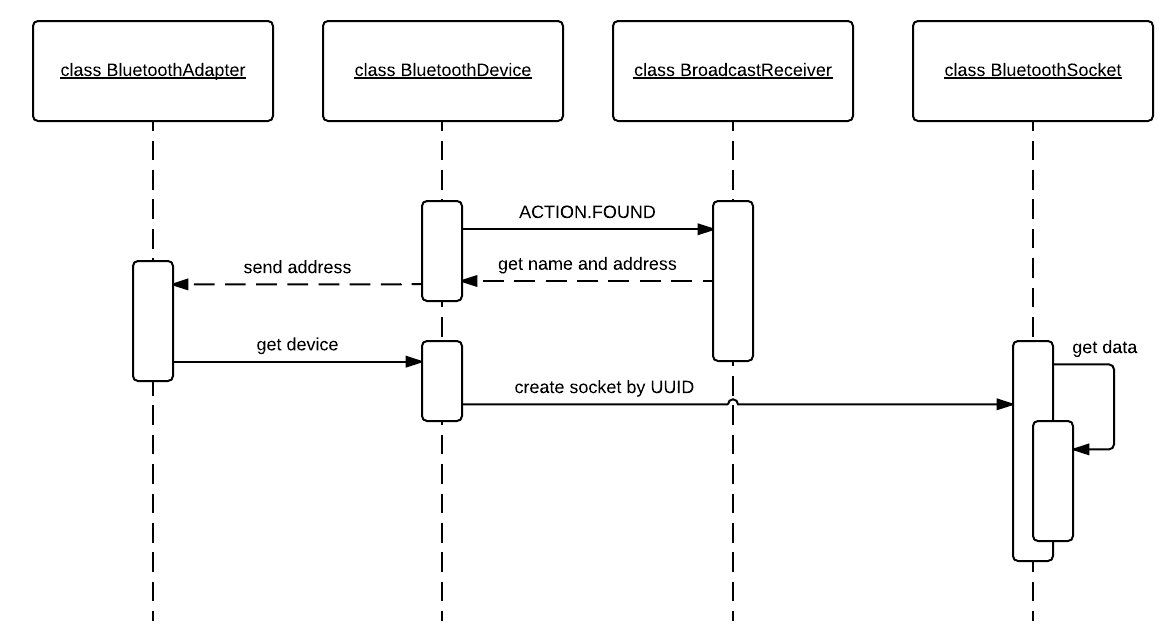
\includegraphics[width=0.9\columnwidth]{fig2-2.png}
        \caption{
                \label{fig2-2}
                Android平台蓝牙连接UML时序图
        }
\end{figure}

\subsection{Android系统绘图功能介绍}

在绘制ECG波形时,不可避免地要接触到Android系统的绘图功能。在Android系统中,View类承载了界面绘制的功能。诸如按钮(Button类)、文本(TextView类)和界面布局(各种Layout类)都以View作为基类。一个Android活动(Activity)通过获取View类来生成界面并且展示给用户,从而产生了使用者最终看到的画面。作为绘制界面的基石,View类自然实现了可以自定义绘制的方法onDraw()。但View类的onDraw操作必须发生在主线程中,所以更新View类的时候,主线程必然是阻塞的,应用程序不会对用户的操作做出回应。这时,如果View更新过程超过5秒,耗时的更新操作还可能引发应用程序未响应的错误(Application Not Responding,ANR)从而强制停止该程序。

使用SurfaceView类绘制图形可以解决这个问题。顾名思义,该类是包含了一个“表面(Surface)”的View类(事实上SurfaceView确实继承了View类)。SurfaceView绘图时,向“表面”,也即真正显示的区域提交的内容和绘画处理的内容可以是不同步的,即该类允许在后台进程中分别进行图像绘制和图像预处理(如加载一个JPEG文件)。因此在图像不更新时,可以先将下一次的绘图预处理,加快下次的显示时间。同时,该类还允许使用者通过重写一个回调函数来获取SurfaceView类对象的状态,并进行相应操作(如初始化绘图线程和销毁绘图线程)。

\begin{figure}[htbp]
 \centering
        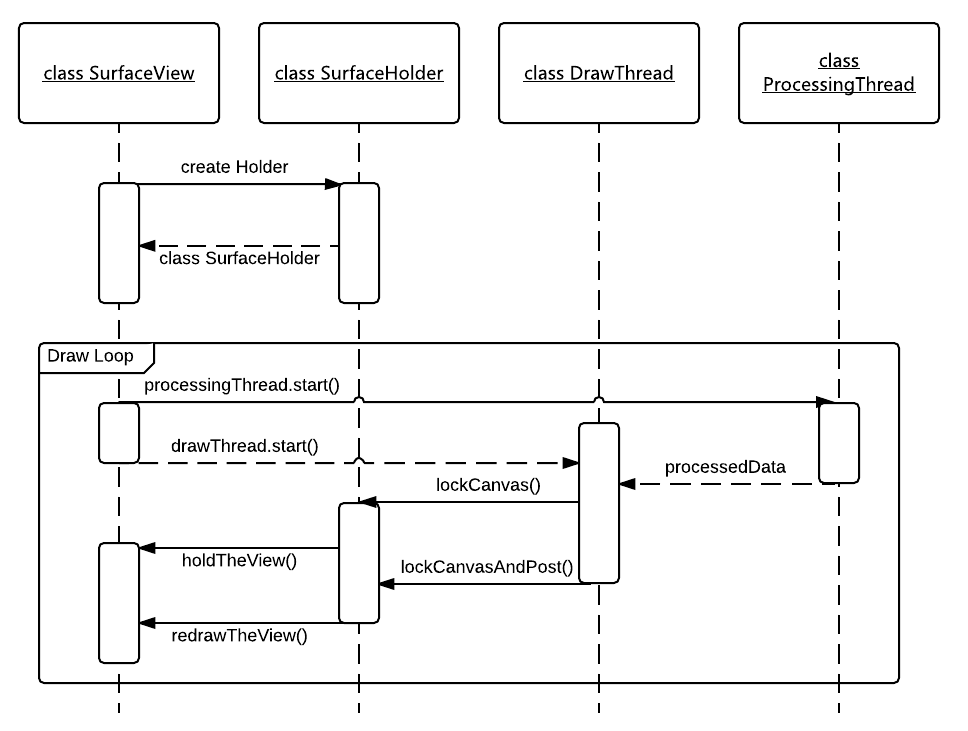
\includegraphics[width=0.9\columnwidth]{fig2-3.png}
        \caption{
                \label{fig2-3}
                Android平台SurfaceView绘图UML时序图
        }
\end{figure}

使用SurfaceView类绘图的过程如图\ref{fig2-3}所示。在实例化各类后,使用SurfaceView获取SurfaceHolder,之后就可以用实现好的回调函数启动图像绘制和处理进程了。这个过程可以循环,以实现图像的持续更新。

\subsection{Android系统SQLite数据库简介}

通过使用Android系统中内嵌的SQLite数据库功能,ECG波形数据可以被方便地组织为SQLite数据库的形态,从而方便数据的查找和输出。

SQLite是一款独立的、无服务器的、零配置的事务型SQL数据库引擎\cite{the_sqlite_development_team_about_????}。SQLite不含服务器端,能够完全嵌入其他程序中,对本地磁盘上的数据库文件进行管理。同时,SQLite的体积十分小巧轻便。一个完全版的SQLite函数库不足500KB,对运行内存的大小也没有苛刻的限制,这使得SQLite十分适合嵌入式平台的应用。作为一款数据库引擎,SQLite十分稳定,很好地保持了数据库事务执行的ACID原则(指原子性、一致性、隔离性和持久性)。

Android自带android.database包,支持SQLite数据库的操作。通过实例化SQLiteDatabase类,能够得到一个SQLite数据库。而通过继承SQLiteOpenHelper类,能够打开已存在的数据库或创建新的数据库。SQLiteOpenHelper还提供了一些回调方法,便于开发者在数据库遭到修改时作出反应。

在Android应用中,提交一个SQLite事务的步骤如下:
\begin{itemize}
\item	调用SQLiteDatabase.beginTransaction()方法开始事务;
\item	进行事务操作(如插入一条记录);
\item	调用SQLiteDatabase.endTransaction()结束事务。
\end{itemize}

同时为方便数据库的查询,Android提供了Cursor类简化诸如查询、遍历数据库等操作。Cursor提供的方法包括返回数据、查询列名、查询列总数、查询数据、移动光标等。

\subsection{本章小结}

本章简要介绍了Android系统的结构、各结构间的关系、概括了各结构是如何协同运行、最终形成一个完整的系统的;介绍了蓝牙技术的基本情况、蓝牙技术所包含的SPP协议是如何在Android平台上得到应用的;最后概述了Android平台中的两个功能性API类:SurfaceView类和SQLiteDatabase类的机制和简要实现方法。

本章所述内容在ECG监测与记录应用的实现中均有涉及,并且构成了应用的几个主要类中的重要部分。可以说,本章介绍的内容可视为应用的主要结构。正因为不同内容所对应的是应用中需要对应的不同现实对象(如Bluetooth相关类对应了有关蓝牙设备的操作、SurfaceView对应了绘图区、SQLiteDatabase对应了ECG数据库等),本应用开发过程严格遵循”面向对象”的原则才得以贯彻,并且其合理性也更能得到印证。


